\section{2-Way Join}
An initial analysis comparing the correlation between Grade and Benchmark data requires a 2-way join between the Grades and Benchmarks datasets. To achieve this, two nETL tasks were run to extract the CSV data (the ``Grades.CSV'' and ``Benchmarks.CSV'' files) and load rows from these CSV files into CouchDB as documents of type ``grade'' and ``benchmark'' respectively. The JSON configuration file in which both these tasks are defined is included in the appendix at \ref{netl-tasks-1-2-config}. Following loading the data from the CSVs into CouchDB, a Map function is used to produce an index of the CouchDB documents sorted by Student ID, with the guarantee that for every unique student id documents are ordered by type; demographic documents are sorted before Grade documents for for any given student. Knowing the sorted order of documents via the view-index allows for performing the join on data-retrieval. In this retrieval (and joining) is performed via a CouchDB List function (discussed below), with the output in CSV format.

\subsection{nETL Configuration}
The ETL processing of Benchmark data involves an iterative approach of first reading a batch of 10 000 lines from the CSV, performing transformations on each line in the batch, and then loading each batch into CouchDB. On notification that a single batch is loaded successfully into CouchDB, a further 10 000 lines are read from the CSV and processed in the same way. This process continues until the entire CSV has been read and loaded into CouchDB. Batches are loaded into CouchDB via the \textit{\_bulk\_docs}. A list of the progression of transformations applied to each line extracted from each CSV is shown below:

\subsubsection{Task 1 Transformations (Grades)}
\begin{enumerate}
  \item A line is converted into a JavaScript object (which relates directly to the JSON format of CouchDB documents) with the fields:
        \begin{itemize}
          \item DownloadedDate
          \item RegAcadYear
          \item RegTerm
          \item anonIDnew
          \item RegProgram
          \item RegCareer
          \item Degree
          \item DegreeDescr
          \item Subject
          \item Catalog.
          \item Course
          \item CourseSuffix
          \item Session
          \item Percent
          \item Symbol
          \item UnitsTaken
          \item CourseID
          \item CourseDescr
          \item CourseCareer
          \item Faculty
          \item Dept
          \item MaximumCrseUnits
          \item CourseCount
          \item CourseLevel
          \item CESM
          \item Sub-CESM
        \end{itemize}
  \item Lines (now in object form) are filtered on the ``RegCareer'' and ``Course'' fields, where grades achieved for the CSC1015F course taken by students registered as undergrads are considered. Lines that don't meet this attribute are discarded and no further transformations are applied to these line.
  \item An attribute (``type\_'') is then added to each line (that weren't removed in filtering step), and given the value ``grade'' to identify each object as a line of the Grade entity type.
  \item Line attributes are whitelisted. The resultant lines each have the the following attributes:
        \begin{itemize}
          \item type\_
          \item Course
          \item RegAcadYear
          \item anonIDnew
          \item Percent
        \end{itemize}
\end{enumerate}

\subsubsection{Task 2 Transformations (Benchmarks)}
\begin{enumerate}
  \item A line is converted into a JavaScript object with the fields:
        \begin{itemize}
          \item anonIDnew
          \item Career
          \item Citizenship Residency
          \item SA School
          \item Eng Grd12 Fin Rslt
          \item Math Grd12 Fin Rslt
          \item Mth Lit Grd12 Fin Rslt
          \item Adv Mth Grd12 Fin Rslt
          \item Phy Sci Grd12 Fin Rslt
          \item NBT AL Score
          \item NBT QL Score
          \item NBT Math Score
          \item RegAcadYear
        \end{itemize}
  \item Lines are filtered on the ``Career'', ``Citizenship Residency'', and ``anonIDnew'' fields. Only lines for students that attended the CSC1015F course during their undergraduate career and that are either South African citizens or permanent residents are included in the result set. The list of students that attended CSC1015 is derived from the Grade data - this is a manual process since the Grade CSV is small enough that manipulation with Microsoft Excel is possible, and this is only required once (so it's not worth automating).
  \item An attribute (``type\_'') is then added to each remaining line and given the value ``benchmark'' to identify each object as a line of the Benchmark entity type.
  \item Line attributes are whitelisted. The resultant lines each have the the following attributes:
        \begin{itemize}
          \item type\_
          \item anonIDnew
          \item Eng Grd12 Fin Rslt
          \item Math Grd12 Fin Rslt
          \item Mth Lit Grd12 Fin Rslt
          \item Adv Mth Grd12 Fin Rslt
          \item Phy Sci Grd12 Fin Rslt
          \item NBT AL Score
          \item NBT QL Score
          \item NBT Math Score
          \item RegAcadYear
        \end{itemize}
\end{enumerate}

\subsection{MapReduce Functions}
The map function for this analysis is included in the appendix (see \ref{2-way-join-map-function}). Each document passed to the map function is treated according to the logic shown in the activity diagram in Figure \ref{2-way-join-map-fn-diagram}. That is, on Map function execution the ``type\_'' attribute is checked. If the document is a line of the Grades entity, then the key [Student ID, year] is emitted along with a single number for the value - the percent achieved for the course. If the document is a line of the Benchmarks entity, then the key [student ID, 0] is emitted along with an ordered list of 8 values corresponding to values for the fields in the Benchmarks.CSV file:

\begin{itemize}
  \item Gr12 English \%
  \item Gr12 science \%
  \item Gr12 Math \%
  \item Gr 12 Math Lit \%
  \item Gr12 Adv Math \%
  \item NBT AL \%
  \item NBT QL \%
  \item NBT Math \%
\end{itemize}

Normalization of the percentage fields (i.e. ``Percent'' for the Grades entity and the test results in the Benchmarks entity) is done via a nested function within the Map function and according to the logic as discussed in that tables previously. No reduce function is used to achieve this 2-way join. This is because, theoretically, a student should only have a single set of Benchmark results and should only achieve a single grade per course per year. As such there is no need to aggregate output from the Map function (which is done via reduction) before performing the document join via the List function.

\begin{figure}[ht]
    \centering
    \begin{mdframed}
        \centering
        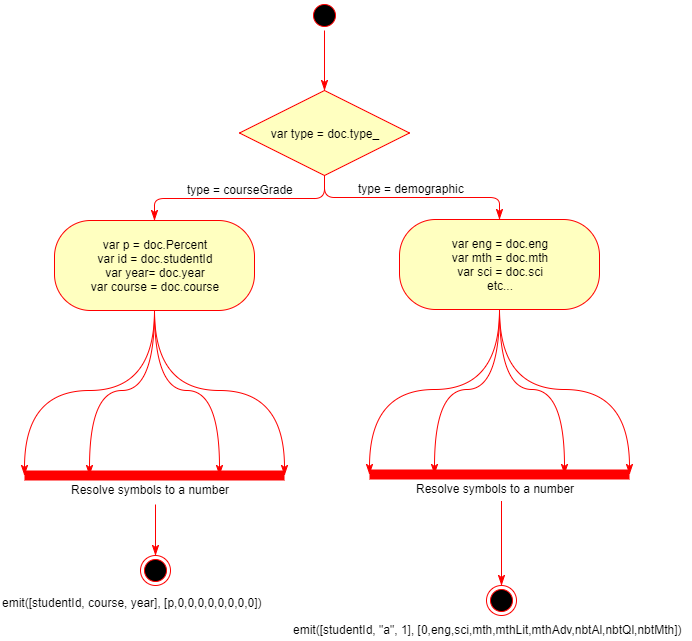
\includegraphics[scale=0.35]{./resources/figures/activity-diagram-1.png}
    \end{mdframed}
    \caption[Result 1 Map function]{\textbf{Figure \ref{result-1-map-fn}: Activity diagram showing logic Map function logic for Results 1 \& 2.} This logic is applied to every document during index calculation (excluding documents with an \_id of ``\_design/*'').}
    \label{result-1-map-fn}
\end{figure}

\subsection{List Function}
The list function is executed via a call to CouchDB's HTTP API. For the project the URI of that function call is \texttt{https://localhost:5984/msc/\_design/2-way-join/\_list/2-way-join-list/ 2-way-join-view?reduce=false}. On invocation the List function opens and scans the index iteratively processing each document (i.e. iteratively processing each student; first a student's demographic document is processed, then a student's grades documents are processed). Figure \ref{fig-2-way-join-list-fn} shows an activity digram representing the logic used to perform the 2-way join in the List function. The logic is wrapped in a CouchDB helper function ``provides'' that accepts two arguments: the type of data the list function will emit (CSV - i.e. plain text data), and a callback that allows uses to create the data that is transformed to the output type. Within the body of the callback the variables `currentStudent', `currentYear', and `currentLine' are set to null. An iteration over the index is initiated using a while loop, with the loop invariant the result of a call to the ``getRow'' function. With the loop invariant equal to true (when a row exists), a check are performed on whether the Student ID of the current row is the same as the Student ID of the previous row. If not, the currentLine variable is emitted via the ``send'' function, and currentStudent is adjusted to be the Student ID from the current row.

Then the type of row being processed is check (whether this key:value pair was emitted from a grade or benchmark document). If from a benchmark document, the scored are added to the currentLine variable and the loop re-executes. If a Grade document, there is a check as to whether the currentYear variable is has the same value as the Year property in the current row. If not, the currentLine variable is emitted and currentYear is adjusted to the new Year value and the loop re-executes.

The currentLine variable is emitted via a subroutine which first checks that the currentLine variable contains data from both the Grades and Benchmarks entity, and then sends a comma-delimited string along a stay-alive network request - this is handled automatically by the HTTP client, which in the case of this project is simply the Google Chrome browser. From a user's perspective, they just watch as a file downloads; the rate at which the file downloads is equal to the rate at which the loop data is output by the send function. Code for the loop function is included in the appendix at \ref{2-Way-join-list-function}.

\begin{figure}[ht]
    \centering
    \begin{mdframed}
        \centering
        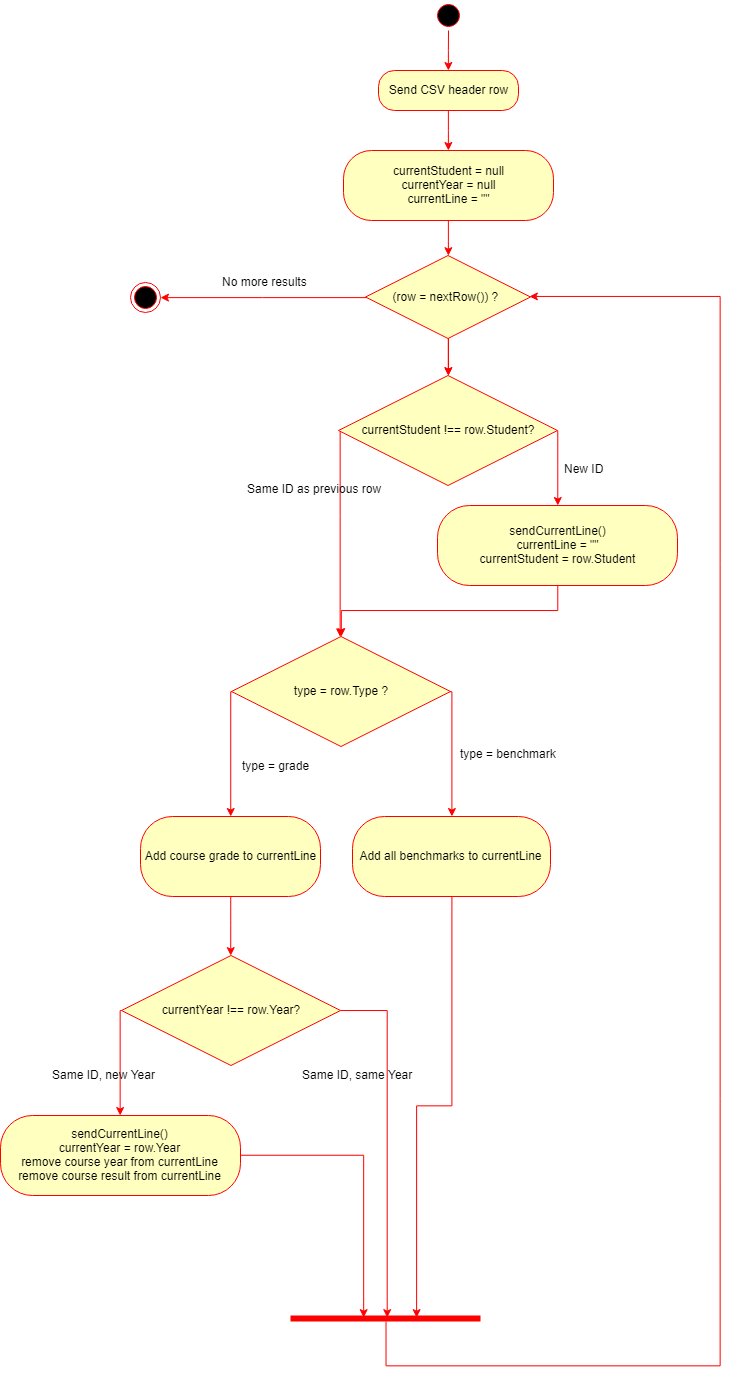
\includegraphics[scale=0.35]{./resources/figures/2-way-join-list.png}
    \end{mdframed}
    \caption[2-Way Join List Function]{\textbf{Figure \ref{2-way-join-list-fn-diagram}: List function logic required to join the Grades and Benchmarks entities.} ...}
    \label{2-way-join-list-fn-diagram}
\end{figure}